
\section{SSH Port Forwarding}
SSH port forwarding is a feature of SSH protocol that allows client and server
to forward additional network connections using base SSH session as a secure,
encrypted and compressed (for improved performance) tunnel.

SSH port forwarding is just a specific SSH-based implementation of a
bigger concept: port forwarding in general helps you get around rigid network
and firewall structures by allowing bi-directional specific network
connectivity via certain network ports. 

SSH port forwarding involves establishing an SSH tunnel between two or more
systems and then configuring the systems to transmit a specified type of
traffic through that connection.

\subsection{Local port forwarding}
Local port forwarding is used to make an external resource available on the
local network.  For example a SQL server only allowing localhost connexion


Local forwarding is used to forward a port from the client machine to the
server machine. Basically, the SSH client listens for connections on a
configured port, and when it receives a connection, it tunnels the connection
to an SSH server. The server connects to a configurated destination port,
possibly on a different machine than the SSH server.

\begin{verbatim}
ssh -L [<local_bind_ip>:]<local_bind_port>:<target_bind_ip|0.0.0.0>:<target_bind_port> <user>@<target_connect_ip>

netstat -antp | grep $L_PORT
lsof -i | egrep '\<ssh\>'
lsof -i -n | egrep '\<ssh\>'

nmap -v -sV -p$L_PORT localhost
\end{verbatim}

{\emph Autossh} is a tool that can be used to create persistent SSH tunnels. The only
prerequisite is that you need to have public key authentication configured
between your systems unless you want to be prompted for a password every time
the connection dies and is re-established.

\subsection{Dynamic port forwarding}

Dynamic port forwarding, also called This is called \emph{SSH tunneling over SOCKS
proxy}, sets up a SOCKS proxy server. You can configure
applications to connect to the proxy and transmit all data through it. The most
common use for this is for private web browsing or to make your connection
seemingly originate from a different country or location.

\begin{figure}
  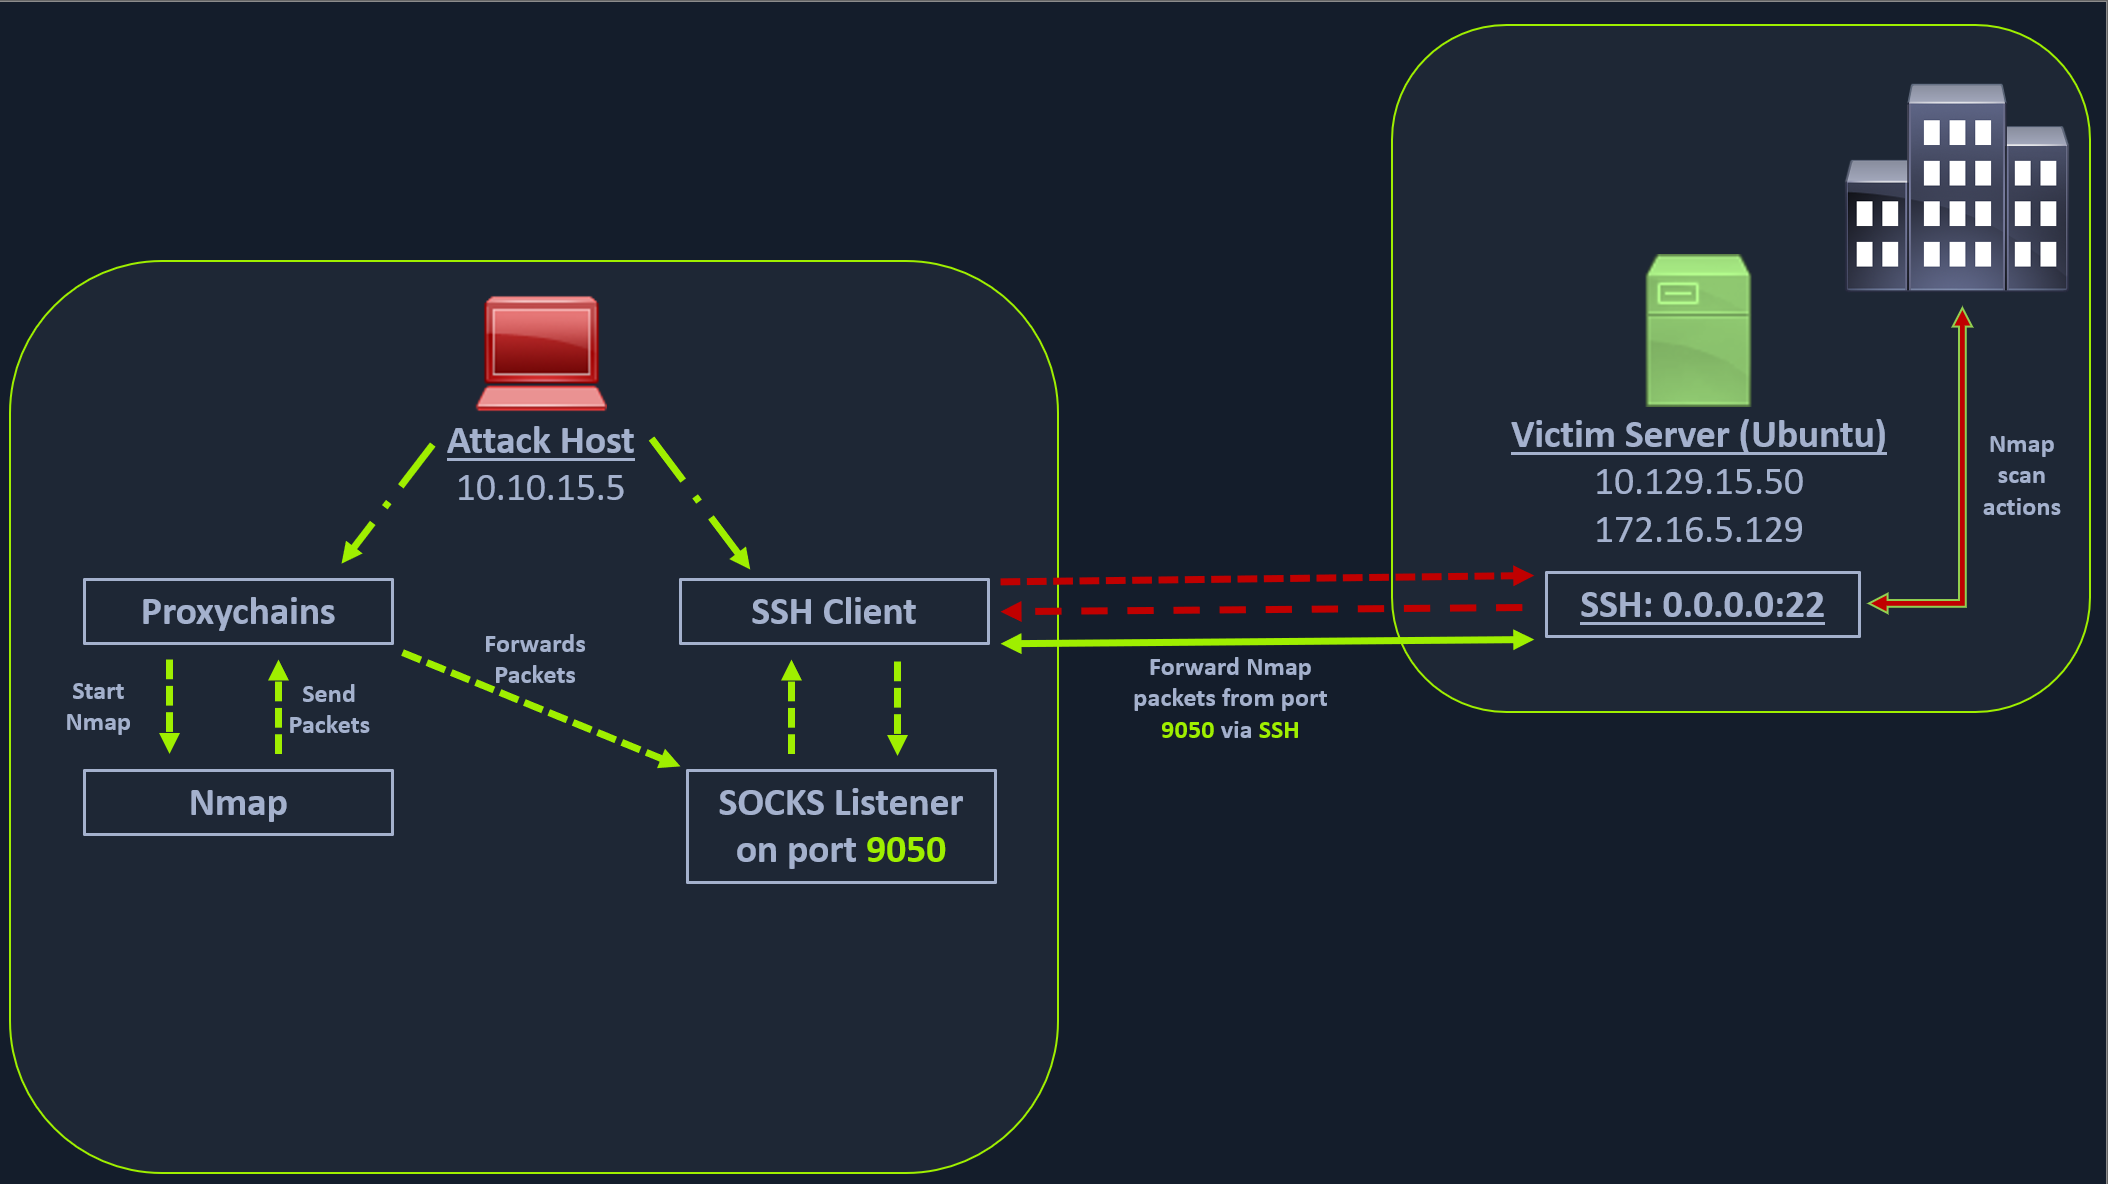
\includegraphics[width=\linewidth]{misc/pivoting/images/dynamic_ssh.png}
  \caption{Dynamic port forwarding}
  \label{fig:dynamic_port_ssh}
\end{figure}


\begin{verbatim}
ssh -D <socks_port> <user>@<target_connect_ip>
\end{verbatim}

\href{https://github.com/haad/proxychains}{proxychains} ProxyChains is a UNIX
program, that hooks network-related libc functions in dynamically linked
programs via a preloaded DLL and redirects the connections through SOCKS4a/5 or
HTTP proxies.

edit \verb+/etc/proxychains.conf+:
\begin{verbatim}
socks5 	127.0.0.1 <socks_port>
\end{verbatim}

Then it is possible to route traffic of application not allowing proxy usage
such as nmap metsaploit, xfreerdp
\begin{verbatim}
proxychains nmap -v -sn 172.16.5.1-200
proxychains msfconsole
proxychains xfreerdp /v:$TARGET /u:$LOGIN /p:$PASSWORD
\end{verbatim}

 One more important note to remember here is that we can only perform a
 \emph{full TCP connect} (\verb+sT+) scan over proxychains.

\subsection{Remote port forwarding}

This works by allocating a socket to listen TCP \verb+target_bind_port+ and \verb+target_bind_ip+ (if omited will listen on all IP).  Whenever a connection is made to this port, the connection is forwarded over the secure channel, and a connection is made from the machine to an explicit destination specified by \verb+fwd_host+ and \verb+fwd_port+. 

if no explicit destination was specified, ssh will act as a SOCKS 4/5 proxy and forward connections to the destinations requested by the remote SOCKS client.

Usefull  to get a reverse shell through a pivot tunnel.

see \verb+GatewayPorts+ config.

\begin{verbatim}
ssh -q -R [<target_bind_ip>:]<target_bind_port>:<fwd_host>:<fwd_port> <user>@<target_connect_ip> -vN
\end{verbatim}

\subsection{Dynamic Remote port forwarding}
Since release 7.6, if \verb+<fwd_host>:<fwd_port>+ is not specified ssh will act as a SOCKS 4/5 proxy  and  forward connections to the destinations requested by the remote SOCKS client. 

So if the \verb+target_bind_ip+ is not speficied (or equals to \verb+target_connect_ip+  we can performe a "reverse dynamic port forward" from the attacking machine.

\begin{verbatim}
ssh -q -R [<target_bind_ip>:]<target_bind_port> <user>@<target_connect_ip> -vN
\end{verbatim}


\subsection{SSH Server-Side Config}
The \verb+AllowTcpForwarding+ option in the OpenSSH server configuration file
must be enabled on the server to allow port forwarding. By default, forwarding
is allowed. Possible values for this option are \verb+yes+ or \verb+all+ to
allow all TCP forwarding, \verb+no+ to prevent all TCP forwarding, \verb+local+
to allow local forwardings, and \verb+remote+ to allow remote forwardings.

Another option of interest is \verb+AllowStreamLocalForwarding+, which can be
used to forward Unix domain sockets. It allows the same values as
AllowTcpForwarding. The default is \verb+yes+.

The \verb+GatewayPorts+ configuration option also affects remote port
forwardings. Possible values were \verb+no+ (only local connections from server
host allowed; default), \verb+yes+ (anyone on the Internet can connect to
remote forwarded ports), and \verb+clientspecified+ (client can specify an IP address that can connect, anyone can if not specified).


\verb+PermitOpen+ can be used to specify the destinations to which port forwarding is allowed. If you only want to allow forwarding to certain IP addresses or hostnames, use this directive. 

\subsection{Low latency}

The only real problem that arises with SSH port forwarding is that there is
usually a bit of latency.  The problem becomes more apparent when doing
network-intensive activities, especially with port forwarding set up as a SOCKS proxy server.

The reason for the latency is because SSH is tunneling TCP over TCP. This is a
terribly inefficient way to transfer data and will result in slower network
speeds.

There is a program called \href{https://github.com/sshuttle/sshuttle}{sshuttle} that corrects the issue. It also remove the
need to configure proxychains.

Sshuttle can be extremely useful for automating the execution of iptables and adding pivot rules for the remote host.

iTo use sshuttle, specify the option \verb+-r+ to connect to the remote machine
with a username and password. Then we include the network or IP we want to
route through the pivot host (for example the network 172.16.5.0/23).

With this command, sshuttle creates an entry in our iptables to redirect all
traffic to the 172.16.5.0/23 network through the pivot host.

\begin{verbatim}
sudo sshuttle -r $USER@RIP -x 172.16.5.0 -vv
\end{verbatim}
